\documentclass{article}
\usepackage{cancel}
\usepackage{graphicx}
\usepackage{soul}
\usepackage[fontsize=14pt]{fontsize}
\usepackage{geometry}
\geometry{left=1in,right=1in,top=1in,bottom=1in}

\begin{document}
	
	\title{Simple\\Numbers and Counting\\Course\\
		\begin{center}
			
\includegraphics[width=4em]{ApS_logo.png}
		\end{center}
		\begin{normalsize}Tutoring Centre Ferndale \end{normalsize}}
	\author{}
	\date{\today}
	
\maketitle

\newpage

\section*{Mathematics} Mathematics is all the ways of handling any sort of numbers or shapes or patterns, and how to solve problems with them. It is a Greek word that originally meant all learning. Mathematics helps us to understand the world so that we can solve problems in the best possible way. It is a big subject that covers lots of different topics.\\

Usually mathematics is just called 'maths' for short (or 'math' in the US.)

\begin{enumerate}
\item What is mathematics?
\item Use it in a sentence.

\subsection*{Arithmetic} Arithmetic is all the ways of handling things that can be counted or numbered. It's a Greek word that means ways of counting. Learning arithmetic well makes learning the rest of maths so much easier.

\item What is arithmetic?
\item Use it in a sentence.
\item Why might it be useful to learn arithmetic?

\newpage

\subsubsection*{Symbol}
A symbol is a thing that has been given a meaning. A symbol stands for or represents something.

\item What is a symbol?
\item What is an example of a symbol?

\subsubsection*{Number}
A number is the idea of an amount or quantity of something or the symbol that stand for it.

\item What is a number?
\item Use it in a sentence.

\paragraph{Numeral}
A numeral is the word or symbol that stands for a number. "Four" and "4", "Twenty seven" and "27", are all numerals.

\item What is a numeral.
\item Use it in a sentence.

\paragraph{Digit}
A digit is a finger. Because people count on their fingers, 0, 1, 2, 3, 4, 5, 6, 7, 8 and 9 are also called digits.

Digits are numerals and they can be put together to make larger numerals. "2" is a numeral with one digit, and "23" is a numeral made up of two digits.

\item What is a digit?
\item Use it in a sentence.

\paragraph{Figure}

A figure is a shape or outline of something. The outline of a person's body is known as their figure, for example, and diagrams in books are sometimes called figures.

0, 1, 2, 3, 4, 5, 6, 7, 8 and 9 are all different shapes so they are called figures. Figures can also mean numbers generally and not just single figures.

Someone might want to "figure it out" meaning they will work with numbers or that they will just think about how to solve some problem.

\item What is a figure?
\item Use it in a sentence.

\subsection*{Count}
Count means to say the names of the numbers one after the other and note each thing as you do to find out how many there are.

\item What is counting?
\item Use it in a sentence.

\subsubsection*{Numbering} To number things means to put a number on each thing as it is counted. The chapters of a book are numbered chapter 1, chapter 2, chapter 3, and so on. Numbering also mean to give the result of a count. You could say that the number of students in the class is 20.

\item What does numbering something mean?
\item What are five things that have been numbered?

\newpage

\section*{Natural Numbers}
Natural means things that are in the natural world, which is the real or physical world. Natural numbers are the numbers that are used for counting things, as in "I have six ducks," or for ordering things, as in "the third duck quacked."

Natural numbers do not include zero.

\item What does 'natural' mean?
\item What is a natural number?

\section*{Whole Numbers}
Whole means the entire thing and not just a part. Whole numbers count whole things.

They are natural numbers, but whole numbers do include zero.

\item What does 'whole' mean?
\item What are whole numbers?

\newpage

\subsection*{Cardinal (Counting) Numbers}
Cardinal means main or most important. The four main directions (north, south, east and west) are called the cardinal directions, for example. 

Natural numbers or whole numbers, when they are used for counting things, are called cardinal numbers, or just counting numbers.

\item What does 'cardinal' mean?
\item What are cardinal numbers?
\item What are counting numbers?

\subsection*{Ordinal Numbers}
Ordinal means having to do with the order that things are in.

Natural numbers or whole numbers, when they give the order of things, are called ordinal numbers.

Counting things as first, second, third, fourth, fifth, and so on, is ordinal numbering.

Pointing to the third ("$3{^{\textrm{rd}}}$") duck in a line of ducks uses an ordinal number.

\item What does 'ordinal' mean?
\item What are ordinal numbers?

\newpage

\section*{Tallies} Tallies are the simplest sort of numeral. For most of human history there were no other numbers. There were just a mark made for each things that was being counted. Tally is an old word for a stick, and a tally was originally a stick with notches cut into it.

A tally looks like this: $\cancel{||||}\ \cancel{||||}\ \cancel{||||}\ |||.$ Every fifth mark is drawn across the last four marks to make the number easier to see.

\item What is a tally?
\item Make a tally of your pens and pencils.

\subsection*{Scores}
A score is a scratch mark, and a score is also 20 of something. That comes from making a mark for every 20 of something being counted. Scores in games are named from keeping a count this way. A famous American speech starts with "Four score and seven years ago..." meaning 87 years ago.

\item What is a score?
\item Use it in a sentence.

\newpage

\section*{Roman Numerals} The Roman Empire ruled most of Europe, and large parts of Africa and Asia, for several centuries about 2000 years ago. Roman numerals and many of their words are still used today.\\

Roman numerals use I for 1, V for 5, X for 10, L for 50, C for 100, D for 500, and M for 1000. The V is said to be a shorthand for a spread hand with 5 fingers and the X is said to be two Vs on top of each other.\\

XVIII in Roman numerals is shorter and easier to read and write than $\cancel{||||}\ \cancel{||||}\ \cancel{||||}\ |||$ as a tally.\\

A smaller amount is written either before or after the larger one, indicating that much more or less. That makes them even shorter to write. For example, XI means 11 because 11 is 1 more than  10, and IX means 9 because 9 is 1 less than 10.\\

Counting in Roman numerals is I II III IV V VI VII VIII IX X XI XII XIII XIV XV… and so on.\\

\newpage

Here are the Roman Numerals from 1 to 100:
\begin{center}
\scriptsize
\renewcommand*{\arraystretch}{1.4}
		\begin{tabular}{rlrlrlrlrl}
			1  & I      & 2  & II      & 3  & III      & 4  & IV     & 5  & V    \\
			6  & VI     & 7  & VII     & 8  & VIII     & 9  & IX     & 10 & X    \\
			11 & XI     & 12 & XII     & 13 & XIII     & 14 & XIV    & 15 & XV   \\
			16 & XVI    & 17 & XVII    & 18 & XVIII    & 19 & XIX    & 20 & XX   \\
			21 & XXI    & 22 & XXII    & 23 & XXIII    & 24 & XXIV   & 25 & XXV  \\
			26 & XXVI   & 27 & XXVII   & 28 & XXVIII   & 29 & XXIX   & 30 & XXX  \\
			31 & XXXI   & 32 & XXXII   & 33 & XXXIII   & 34 & XXXIV  & 35 & XXXV \\
			36 & XXXVI  & 37 & XXXVII  & 38 & XXXVIII  & 39 & XXXIX  & 40 & XL   \\
			41 & XLI    & 42 & XLII    & 43 & XLIII    & 44 & XLIV   & 45 & XLV  \\
			46 & XLVI   & 47 & XLVII   & 48 & XLVIII   & 49 & XLIX   & 50 & L    \\
			51 & LI     & 52 & LII     & 53 & LIII     & 54 & LIV    & 55 & LV   \\
			56 & LVI    & 57 & LVII    & 58 & LVIII    & 59 & LIX    & 60 & LX   \\
			61 & LXI    & 62 & LXII    & 63 & LXIII    & 64 & LXIV   & 65 & LXV  \\
			66 & LXVI   & 67 & LXVII   & 68 & LXVIII   & 69 & LXIX   & 70 & LXX  \\
			71 & LXXI   & 72 & LXXII   & 73 & LXXIII   & 74 & LXXIV  & 75 & LXXV \\
			76 & LXXVI  & 77 & LXXVII  & 78 & LXXVIII  & 79 & LXXIX  & 80 & LXXX \\
			81 & LXXXI  & 82 & LXXXII  & 83 & LXXXIII  & 84 & LXXXIV & 85 & LXXXV\\
			86 & LXXXVI & 87 & LXXXVII & 88 & LXXXVIII & 89 & LXXXIX & 90 & XC   \\
			91 & XCI    & 92 & XCII    & 93 & XCIII    & 94 & XCIV   & 95 & XCV  \\
			96 & XCVI   & 97 & XCVII   & 98 & XCVIII   & 99 & XCIX   & 100& C    \\
		\end{tabular}
\end{center}
\begin{center}
    \scriptsize
    I = 1, V = 5, X = 10, L = 50, C = 100, D = 500, M = 1000
\end{center}

\newpage

\item What does 'Roman' mean?
\item Find Rome on a map.
\item What was the Roman Empire?
\item What are Roman numerals?
\item Are Roman numerals better than tallies? Why?
\item Have you seen Roman numerals before? Where?
\item Write the number of things on your table right now in Roman numerals.
\item Write from 1 to 20 using Roman numerals.
\item What is MMXXIV ?

\newpage

\section*{Arabic Numerals}
The numerals that we use today, 0 1 2 3 4 5 6 7 8 9, are called Arabic numerals. They came to Europe though the Arab world and they are originally from India. They first appeared in Europe in the $10^{\textrm{th}}$ century but they weren't in common use until around the $15^{\textrm{th}}$ century.\\
\begin{center}
{\Huge \textbf{0 1 2 3 4 5 6 7 8 9}}
\end{center}

The style of these numerals can vary. Some people write four closed at the top and some people leave it open.

\begin{center}
    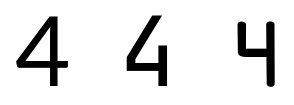
\includegraphics[width=4em]{numeral 4.png}
\end{center}
Some people write nine with a straight line and some people use a curve.
\begin{center}
    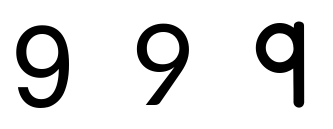
\includegraphics[width=4em]{numeral 9.png}
\end{center}

Also, so that zero isn't confused with the letter O, sometimes 0 is written with a line through it, and 7 sometimes has a line through it as well so that it isn't confused with a 1.

$${\Large \cancel{\textbf{0}} \hspace{2em} \textrm{\st{\textbf{7}}}}$$

\item In your own words, what is 'Arabic'?
\item Make a sentence using the word 'Arabic.'
\item In your own words, what is an Arabic numeral?
\item Write out the Arabic numerals.

\subsection*{The Place-Value System}
Until Arabic numerals came to Europe, there were only Roman numerals and systems of tallies and counting stones.

The new Arabic numerals were used in a different and much more powerful way.\\

A Roman number only ever stood for that one amount. A Roman V only ever meant five of something, even when it was part of a larger number containing other Roman numerals.\\

The amount that one of these Indian numerals stood for, though, when it was part of a larger number with more than one numeral, changed depending on it’s position in that number. A ‘5’ could mean five of something, or fifty, or five hundred, depending on it’s position.\\

This is the place-value system. The value of any digit in a number depends on it’s place in that number. Each digit is read not just as itself but it's value is ten times more than the digit to it’s right.\\

\subsubsection*{The Base}
The number that is chosen to multiply each position by is known as as the base. Any number can be used as a base.

\paragraph{Decimal Base}
We usually use the number 10 as the base, which is why most numbers that you see are called decimal numbers. Decimal means having to do with 10.

In decimal numbers, the digit at the right of a number is just itself, but the digit to its left has 10 times its value, and the next digit to the left has 100 times its value, and so on.\\

123 is short for $(1 \times 10 \times 10) + (2 \times 10) + (3 \times 1)$.\\

A tally of $\cancel{||||}\ \cancel{||||}\ \cancel{||||}\ \cancel{||||}\ \cancel{||||}\ \cancel{||||}\ \cancel{||||}\ \cancel{||||}\ \cancel{||||}\ \cancel{||||}\ \cancel{||||}\ \cancel{||||}\ \cancel{||||}\ \cancel{||||}\ \cancel{||||}\ \cancel{||||}\ \cancel{||||}\: \cancel{||||}\ \cancel{||||}\ \\ \cancel{||||}\ \cancel{||||}\ \cancel{||||}\ \cancel{||||}\: \cancel{||||}\ |||$ could be written more briefly as CXXIII in Roman numerals, or simply as 123 in Hindu-Arabic numerals.

\item What does 'place-value' mean?
\item What does each of the digits in the number '234' mean?
\item What does 'base' mean in the place-value system?
\item What does 'decimal' mean?
\item Why are the numbers that we mostly use called decimal numbers?

\newpage

\section*{Names of Large Numbers}
Large numbers have special names.

\begin{itemize}
\item A hundred is ten tens, written as 100.
\item A thousand is ten hundreds, 1000.
\item A million is a thousand thousand, 1000,000.
\item A billion is a thousand million, 1000,000,000.\\
(The 'bi-', meaning two, in 'billion' is because a billion once meant a million million.)
\item A trillion is a thousand billion, 1000,000,000,000.\\
(The 'tri-', meaning three, in 'trillion' is because a trillion once meant a million million million.)
\item A googol is 1 followed 100 zeroes, and is where the internet company Google got its name.
\end{itemize}

\subsection*{Commas}
To make large decimal numbers easier to read, every third digit is separated by a comma. Then you can read off each group of digits as hundreds, thousands, millions, and so on.\\

Is the first digit of 1234567 millions? tens of millions?\\

Written as 1,234,567 it is easier to see that it is millions.\\

Large numbers are read from the left, in groups of three digits.\\

123,456,987,654,321 is read as 123 trillion, 456 billion, 987 million, 654 thousand, 3 hundred and 21.\\

\item How are commas used in writing large decimal numbers?
\item Write a decimal number with 8 digits, and then put commas every 3 places to make it easier to read.
\item Now read off your large number.

\newpage

\section*{Fractions}
A fraction is a part of a whole number that has been broken into equal-sized parts. They are written as the number of parts and the number of parts that the whole number was broken into. $\frac{3}{4}$ is a fraction where a whole number has been broken into 4 parts and we have 3 of those parts.

\item In your own words, what is a fraction?
\item Write an examples of a fraction.

\subsection*{Decimal Fractions}
Fractions can also be written as decimal numbers using the place-value system. Just as each digit is ten times the value of the digit to its right, each digit is also a tenth of the value of the digit to its left.

\paragraph{The Decimal Point}
To write a decimal fraction, the decimal point is a full stop that marks where the whole number part of a number ends and where the fractional part starts.

Fractions written as decimal numbers are called decimal fractions. They are usually the answers given by calculators, and they are the answers that you get when doing division by hand.

Decimal numbers are sometimes just called decimals, and decimal fractions are also often just called decimals.

$$12.34 = 10 + 2 + \frac{3}{10} + \frac{4}{100}$$

For a number less than 1, the zero in the units position is still written to make it clear that the number is a fraction. You write 0.25, not just .25.

\item What is a decimal point?
\item In your own words, what are decimal fractions?
\item With a calculator, find $3 \div 4$ and write down what the digits of that answer mean.

\end{enumerate}
\end{document}
